%
% ---------------------------------------------------------------
% Copyright (C) 2012-2018 Gang Li
% ---------------------------------------------------------------
%
% This work is the default powerdot-tuliplab style test file and may be
% distributed and/or modified under the conditions of the LaTeX Project Public
% License, either version 1.3 of this license or (at your option) any later
% version. The latest version of this license is in
% http://www.latex-project.org/lppl.txt and version 1.3 or later is part of all
% distributions of LaTeX version 2003/12/01 or later.
%
% This work has the LPPL maintenance status "maintained".
%
% This Current Maintainer of this work is Gang Li.
%
%

\documentclass[
 size=14pt,
 paper=smartboard,  %a4paper, smartboard, screen
 mode=present, 		%present, handout, print
 display=slides, 	% slidesnotes, notes, slides
 style=tuliplab,  	% TULIP Lab style
 pauseslide,
 fleqn,leqno]{powerdot}


%我自己增加的两端对其用
\usepackage{ragged2e}
\renewcommand{\raggedright}{\leftskip=0pt \rightskip=0pt plus 0cm}


\usepackage{cancel}
\usepackage{caption}
\usepackage{stackengine}
\usepackage{smartdiagram}
\usepackage{attrib}
\usepackage{amssymb}
\usepackage{amsmath} 
\usepackage{amsthm} 
\usepackage{mathtools}
\usepackage{rotating}
\usepackage{graphicx}
\usepackage{boxedminipage}
\usepackage{rotate}
\usepackage{calc}
\usepackage[absolute]{textpos}
\usepackage{psfrag,overpic}
\usepackage{fouriernc}
\usepackage{pstricks,pst-3d,pst-grad,pstricks-add,pst-text,pst-node,pst-tree}
\usepackage{moreverb,epsfig,subfigure}
\usepackage{color}
\usepackage{booktabs}
\usepackage{etex}
\usepackage{breqn}
\usepackage{multirow}
\usepackage{natbib}
\usepackage{bibentry}
\usepackage{gitinfo2}
\usepackage{siunitx}
\usepackage{nicefrac}
%\usepackage{geometry}
%\geometry{verbose,letterpaper}
\usepackage{media9}
\usepackage{animate}
%\usepackage{movie15}
\usepackage{auto-pst-pdf}

%\usepackage{breakurl}
\usepackage{fontawesome}
\usepackage{xcolor}
\usepackage{multicol}



\usepackage{verbatim}
\usepackage[utf8]{inputenc}
\usepackage{dtk-logos}
\usepackage{tikz}
\usepackage{adigraph}
%\usepackage{tkz-graph}
\usepackage{hyperref}
%\usepackage{ulem}
\usepackage{pgfplots}
\usepackage{verbatim}
\usepackage{fontawesome}


\usepackage{todonotes}
% \usepackage{pst-rel-points}
\usepackage{animate}
\usepackage{fontawesome}

\usepackage{listings}
\lstset{frameround=fttt,
frame=trBL,
stringstyle=\ttfamily,
backgroundcolor=\color{yellow!20},
basicstyle=\footnotesize\ttfamily}
\lstnewenvironment{code}{
\lstset{frame=single,escapeinside=`',
backgroundcolor=\color{yellow!20},
basicstyle=\footnotesize\ttfamily}
}{}


\usepackage{hyperref}
\hypersetup{ % TODO: PDF meta Data
  pdftitle={Kaggle sildes},
  pdfauthor={Wang Mingxi},
  pdfpagemode={FullScreen},
  pdfborder={0 0 0}
}


% \usepackage{auto-pst-pdf}
% package to show source code

\definecolor{LightGray}{rgb}{0.9,0.9,0.9}
\newlength{\pixel}\setlength\pixel{0.000714285714\slidewidth}
\setlength{\TPHorizModule}{\slidewidth}
\setlength{\TPVertModule}{\slideheight}
\newcommand\highlight[1]{\fbox{#1}}
\newcommand\icite[1]{{\footnotesize [#1]}}

\newcommand\twotonebox[2]{\fcolorbox{pdcolor2}{pdcolor2}
{#1\vphantom{#2}}\fcolorbox{pdcolor2}{white}{#2\vphantom{#1}}}
\newcommand\twotoneboxo[2]{\fcolorbox{pdcolor2}{pdcolor2}
{#1}\fcolorbox{pdcolor2}{white}{#2}}
\newcommand\vpspace[1]{\vphantom{\vspace{#1}}}
\newcommand\hpspace[1]{\hphantom{\hspace{#1}}}
\newcommand\COMMENT[1]{}

\newcommand\placepos[3]{\hbox to\z@{\kern#1
        \raisebox{-#2}[\z@][\z@]{#3}\hss}\ignorespaces}

\renewcommand{\baselinestretch}{1.2}


\newcommand{\draftnote}[3]{
	\todo[author=#2,color=#1!30,size=\footnotesize]{\textsf{#3}}	}
% TODO: add yourself here:
%
\newcommand{\gangli}[1]{\draftnote{blue}{GLi:}{#1}}
\newcommand{\shaoni}[1]{\draftnote{green}{sn:}{#1}}
\newcommand{\gliMarker}
	{\todo[author=GLi,size=\tiny,inline,color=blue!40]
	{Gang Li has worked up to here.}}
\newcommand{\snMarker}
	{\todo[author=Sn,size=\tiny,inline,color=green!40]
	{Shaoni has worked up to here.}}

%%%%%%%%%%%%%%%%%%%%%%%%%%%%%%%%%%%%%%%%%%%%%%%%%%%%%%%%%%%%%%%%%%%%%%%%
% title
% TODO: Customize to your Own Title, Name, Address
%
\title{The Final Report}
\author{
Wang Mingxi
\\
\\Jilin University
\\College of Computer Science and Technology
}
\date{\gitCommitterDate}
%\date{\today} %暂时手写改动

% Customize the setting of slides
\pdsetup{
% TODO: Customize the left footer, and right footer
rf=\href{http://www.tulip.org.au}{
Last Changed by: \textsc{\gitCommitterName}\ \gitVtagn-\gitAbbrevHash\ (\gitAuthorDate)
%Last Changed by: \textsc{Mingxi Wang}\ \gitVtagn-\gitAbbrevHash\ (\today)
},
cf={flip00-kaggle},
}


\begin{document}

\maketitle

%\begin{slide}{Overview}
%\tableofcontents[content=sections]
%\end{slide}


%%==========================================================================================
%%
\begin{slide}[toc=,bm=]{Overview}
\tableofcontents[content=currentsection,type=1]
\end{slide}
%%
%%==========================================================================================


\section{Research motivation and context}

%%==========================================================================================
%%
\begin{slide}{Project Objectives}

\begin{itemize}
\item The project analyzed 12 years of crime reports from all of San Francisco's neighborhoods to create a model that can predict crime categories at a given time and place.

\end{itemize}

\begin{center}
	\begin{figure}[htbp]
		\includegraphics[scale=0.4]{./pic/SF.eps}
		\caption{project preview}
	\end{figure}
\end{center}

\end{slide}
%%
%%==========================================================================================

%%==========================================================================================
%%
\begin{slide}{Project background}

\raggedright
Crime is a kind of behavior that does great harm to the society. It brings great loss of life and property to human beings.In modern society, human beings prevent crime through strict judicial means, and research on crime prevention based on sociology, psychology and law.The objective of this project is to quantitatively analyze a data set of nearly 12 years of crime reports from all San Francisco neighborhoods by computer means and to create a model that predicts the type of crime that will occur given information such as time and location.

\end{slide}

\section{Research contents and methods}

%%
%%==========================================================================================
\begin{slide}{Evaluation metric}
%当有多个Kaggle Subject而只想在目录出现一次时,在后面几次Kaggle Subject前加上[toc=,bm=]
	\raggedright
	Multi-class logarithmic loss, which measures that the model output is a probability value between 0 and 1.


\end{slide}

\begin{slide}{Data set preview}
	\begin{itemize}
	\item 878,049 samples, a total of 9 features.
	\end{itemize}
	Date, category, description, day of the week, name of the police district, solution, approximate street address of the crime, longitude, latitude.\\
	\begin{center}
		\begin{figure}[htbp]
			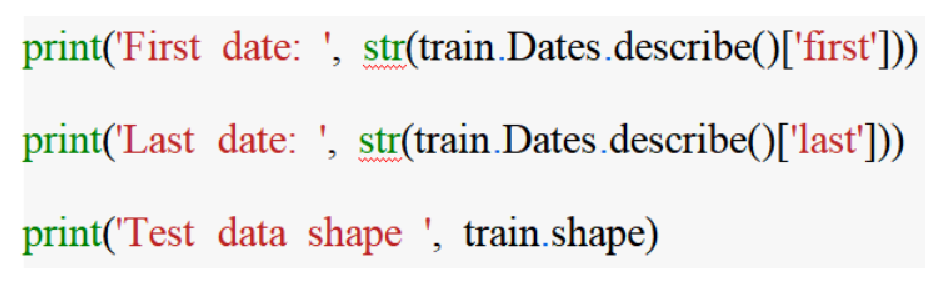
\includegraphics[scale=0.6]{./pic/qmcode1.eps}
			\caption{preview}
		\end{figure}
	\end{center}
	First date:  2003-01-06 00:01:00\\
	Last date:  2015-05-13 23:53:00\\
	Test data shape  (878049, 9)\\
	
	
\end{slide}

\begin{slide}[toc=,bm=]{Data set preview II}
	\begin{itemize}
	\item train.head()
	\end{itemize}
	\begin{center}
		\begin{figure}[htbp]
			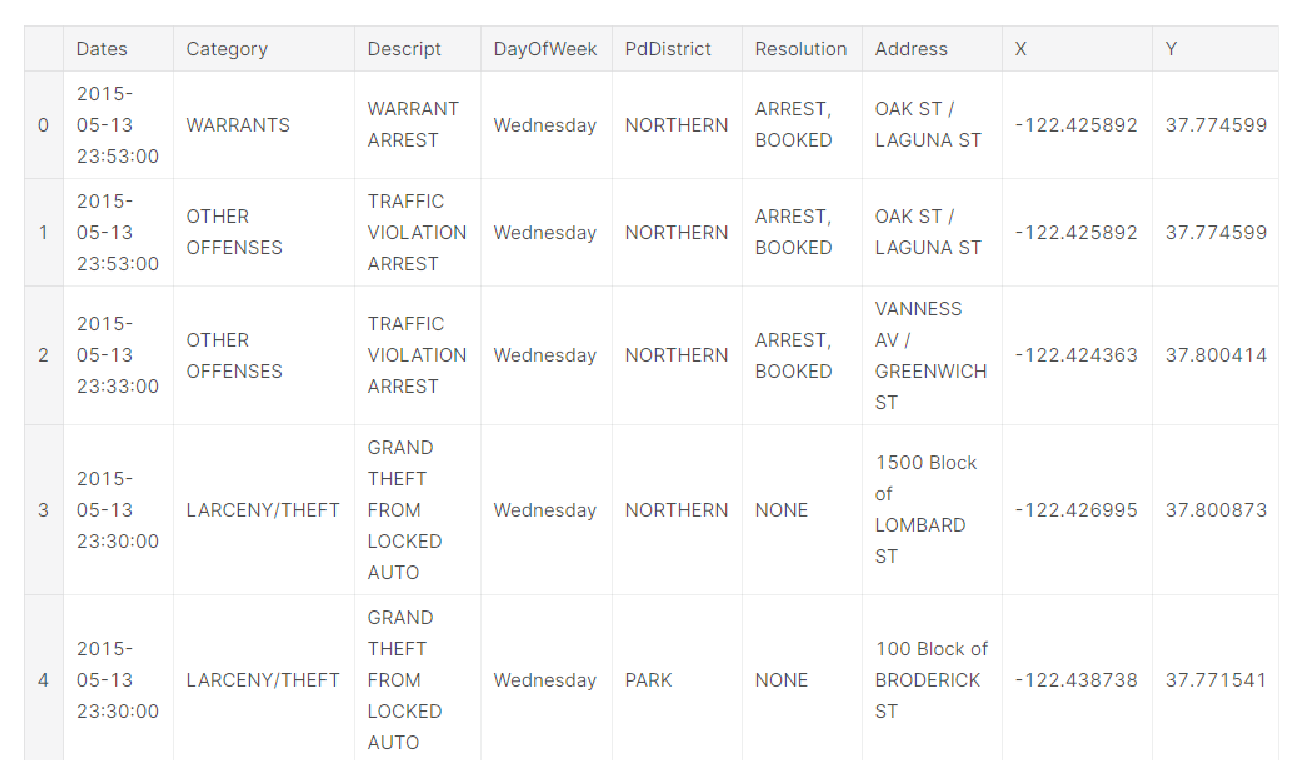
\includegraphics[scale=0.6]{./pic/qmyangben.eps}
			\caption{preview}
		\end{figure}
	\end{center}
\end{slide}

\begin{slide}{Data cleaning}
	\begin{itemize}
		\item There are 2323 duplicate items that need to be removed
	\end{itemize}
		train.duplicated().sum()
	\begin{itemize}
		\item Throw away samples in a range of longitude and latitude (e.g., 50)
	\end{itemize}
	
	
\end{slide}

\begin{slide}{Characteristics of the engineering}
	\begin{center}
		\begin{figure}[htbp]
			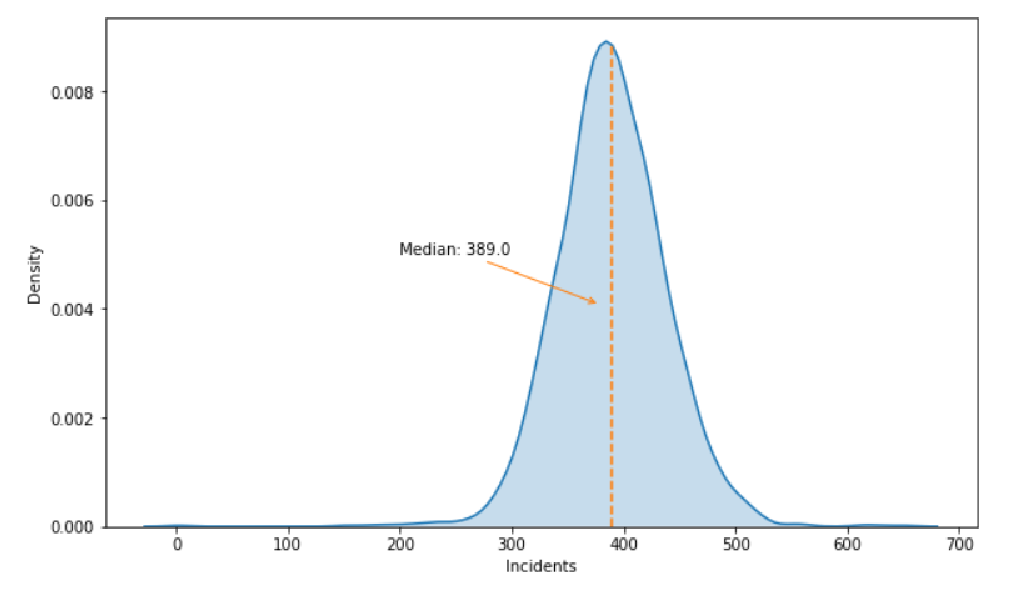
\includegraphics[scale=0.8]{./pic/qmzhengtai.eps}
			\caption{Distribution of number of incidents per day}
		\end{figure}
	\end{center}
	
\end{slide}

\begin{slide}[toc=,bm=]{Characteristics of the engineering II}
Similarly, there was no significant deviation in the frequency of events over the course of the week.
	\begin{center}
		\begin{figure}[htbp]
			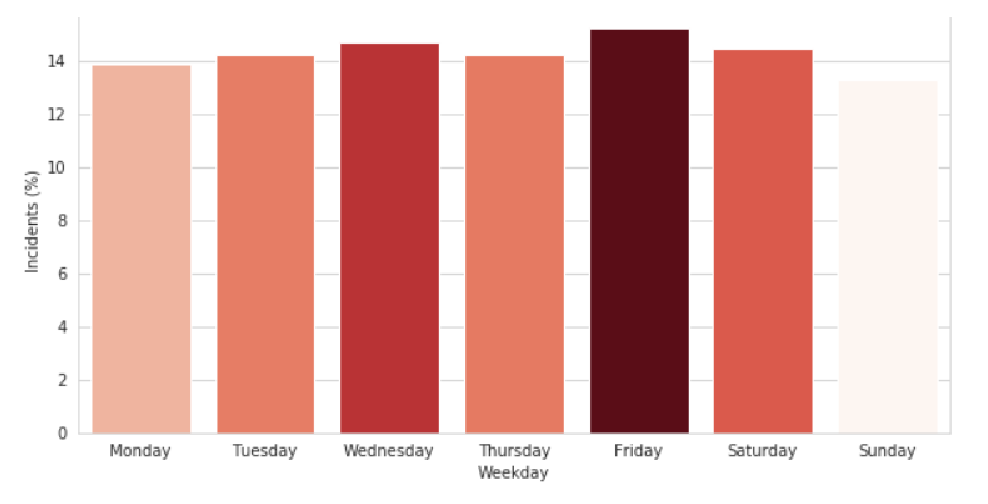
\includegraphics[scale=0.8]{./pic/qmzhifangtu.eps}
			\caption{incidents per Weekday}
		\end{figure}
	\end{center}
	
\end{slide}

\begin{slide}[toc=,bm=]{Characteristics of the engineering III}
A total of 39 discrete categories of incidents were recorded by police stations, the most common being theft (19.91\%), non-criminal cases (10.50\%) and assault (8.77\%)

		\begin{figure}[htbp]
			\includegraphics[scale=0.5]{./pic/qmshuxingtu.eps}
			\caption{incidents per Crime Category}
		\end{figure}
	
\end{slide}

\begin{slide}[toc=,bm=]{Characteristics of the engineering IV}
The chart below shows the average number of incidents per hour for the five crime categories.
Obviously, different crimes occur with different frequencies at different times of the day.
Prostitution, for example, takes place mostly at night, gambling incidents take place from late at night until morning, and burglaries from early morning until afternoon.
As before, this is clear evidence that time parameters will also play an important role.
	
	\begin{figure}[htbp]
		\includegraphics[scale=0.9]{./pic/qmzhexiantu.eps}
		\caption{average number of incidents per hour}
	\end{figure}
	
\end{slide}

\begin{slide}[toc=,bm=]{Characteristics of the engineering V}
	\begin{itemize}
		\item From the "Date" field, we extracted the date, month, year, hours, minutes, days, and days since the first day.
		\item We extracted from the "Address" field whether the event occurred at the intersection or on a building component.
	\end{itemize}
\end{slide}
\begin{slide}{Information coding}
	\raggedright
	The discrete data is converted to a number between 0 and N-1, where N is the number of different values in a list.You can think of it as the number of different values of a feature.
\end{slide}
\begin{slide}{Training model}
	\begin{itemize}
	\item Train 23 Epochs.
	\item Use cross validation to evaluate the quality of our model.\\
	After training, the model obtained:
	\item a cross validation score of 2.46.
	\item it got 2.49 on the test set.
	\end{itemize}
\end{slide}

\section{Architecture of the model}

\begin{slide}{Architecture of the model}
1. Make the decision tree fit the data\\
2. Evaluation model\\
3. Add weight to incorrect samples.\\
4. Select the leaf nodes with the greatest incremental loss for growth.\\
5. Generate the tree at the node in the previous step.\\
6. Go to Step 2 for the cycle\\
\end{slide}

\section{Conclusion}


\begin{slide}{Conclusion}

Conclusion: Based on data analysis, processing and utilization, our model can effectively predict crime types.By using the multi-classification algorithm to analyze the input features and update the model parameters through iterative training, our model can be trained more and more accurately.So as to complete the task of classification prediction.


\end{slide}
%%
%%==========================================================================================

%%==========================================================================================
%%

%%
%%==========================================================================================



%%
%%==========================================================================================


%%==========================================================================================
% TODO: Contact Page
\begin{wideslide}[toc=,bm=]{Contact Information}
\centering
\vspace{\stretch{1}}
\twocolumn[
lcolwidth=0.35\linewidth,
rcolwidth=0.65\linewidth
]
{
% \centerline{
\includegraphics[scale=.2]{tulip-logo.eps}}
}
{
\vspace{\stretch{1}}
Wang Mingxi\\
College of Computer Science and Technology\\
Jilin University, China
\begin{description}
 \item[\textcolor{orange}{\faEnvelope}] \href{mailto:mxwang@tulip.academy}
 {\textsc{\footnotesize{mxwang@tulip.academy}}}

 \item[\textcolor{orange}{\faHome}] \href{http://www.tulip.org.au}
 {\textsc{\footnotesize{Team for Universal Learning and Intelligent Processing}}}
\end{description}
}
\vspace{\stretch{1}}
\end{wideslide}

\end{document}

\endinput
